\documentclass[preprint]{revtex4-1}
\usepackage{graphicx}
\usepackage{epstopdf}
\usepackage{amsmath}
\usepackage{hyperref}
\usepackage{booktabs}
\usepackage{color}

\usepackage{SIunits}
\newcommand{\wstar}{-0.023}
\newcommand{\Qstar}{0.25}

\setlength{\tabcolsep}{10pt}

\newenvironment{sistema}%
  {\left\lbrace\begin{array}{@{}l@{}}}%
  {\end{array}\right.}


\DeclareMathOperator{\erf}{erf}

\begin{document}
\title{Quantitative localisation and sizing of polydisperse colloids from confocal microscopy images}



\author{Mathieu Leocmach} 

\author{Hajime Tanaka}
\affiliation{ {Institute of Industrial Science, University of Tokyo, 4-6-1 Komaba, Meguro-ku, Tokyo 153-8505, Japan} }

\date{Received \today}

\begin{abstract}
We propose a scale-space based method to extract both the individual 3D coordinates and the radii of spherical colloids from confocal microscopy images. According to synthetic and real data, dilute or crowded, particles can be detected correctly without assumption on their sizes, even when particle diameters differ by large factors. Moreover the size of each particle can be estimated within a few percent error (less than $0.3\%$ if the diameter is larger than \unit{5}{px}).
\end{abstract}
\maketitle

\section*{Introduction}
Particle-level confocal microscopy experiments usually access the coordinates of the particles via the algorithm proposed by \citet{Crocker1996}. The original noisy image is blurred by convolution with a Gaussian kernel of width $\sigma$ to yield a soft peak per particle. Local intensity maxima within this blurred image give the coordinates of the particles with pixel resolution. Sub-pixel resolution ($0.1\sim0.3$~pixels error) can be achieved by taking the centre of mass of a neighbourhood around the local maxima. The extension of this algorithm in 3D has been done in two ways: either tracking particles in each confocal plane and reconstructing the results (2D-flavour)~\citep{dinsmore2001tdc}, or full image analysis on three dimensional pictures (3D-flavour)~\citep{vanblaaderen1995rss, Lu2007}.

The choice of the width $\sigma$ of the blurring kernel is critical: if it is too small, then the intensity profile is flat near the centre  of a particle, leading to multiple and ill-localized maxima per particle; if it is too large, then the peaks of nearby particles overlap, leading to shifts in the detected positions, or even fusion of the particles (only one particle detected instead of two). If the colloids are fairly monodisperse one can argue (at least in the 3D-flavour) that there exists a range of possible width where the choice of $\sigma$ has almost no effect on the number of particles detected. Choosing $\sigma$ within this range gives confidence in the localisation results.

However, we found that no such ``good blur width'' exists in our polydisperse sample (see Fig.~\ref{fig:localise}c-h). The detection of smaller particles with small blurring widths leads to the failure in detecting properly the larger particles. This unacceptable failure of the \citet{Crocker1996} algorithm, as well as the want of the particles' radii data, triggered our design of a novel localisation algorithm that would be robust even for a system of finite polydispersity, which is unavoidable in real experiments.

The key notion to detect objects of unknown and possibly diverse sizes in an image is the \emph{scale space}~\cite{Lindeberg1993}. A popular implementation for isotropic objects (or ``blobs'') is the Scale Invariant Feature Transform (\textsc{sift}) of \citet{Lowe2004}. It is often used to match between different images from complex objects consisting of many rigidly linked blobs and further characterised by local histograms~\citep{Lowe2004}. To our knowledge, this method was never used for the quantitative localisation and sizing of independent single-blob objects like spherical colloids.

In the following, we will start by recalling the principle of \textsc{sift}, then explaining our method in the ideal case of an isolated binary ball and then add successively finite dilution, difference in brightness between the particles and distortion by a point-spread function. Finally, we will present the results of our method from real experimental data (see Fig.~\ref{fig:localise}a).

\section*{Principle}

The \textsc{sift} consists in convolving the original image $I$ by Gaussian kernels $g_{\sigma_s}$ of logarithmically increasing widths $\sigma_s$ to obtain a series of blurred images $G_s$
\begin{align}
\forall s>0,\quad G_s = I \star g_{\sigma_s}, \label{eq:gaussian_blur}\\
\intertext{where $\star$ is the convolution operator and}
\forall s>0,\quad \sigma_{s} = 2^{s/n} \sigma_0 ,
\label{eq:sigma_s}
\end{align}
with $n$ a fixed integer. Following \cite{Lowe2004} we use $\sigma_0=1.6$ and $n=3$. Bright objects in the original image appear as bright blobs in the blurred images, and the blobs fuse together as the kernel width increases. This can be seen as a lower and lower-pass filter in the frequency domain. If we take the difference between consecutive blurred images we obtain a comb of band pass filtered versions of $I$: 
\begin{equation}
\forall s>1,\quad DoG_s = G_s - G_{s-1} \label{eq:DoG_s}
\end{equation}
The difference of Gaussians (DoG) response function defined in this way depends on the position in space and on the scale. Bright objects in the original image are detected as local minima in $DoG_s$. Furthermore, the intensity of the response is optimal at a $\sigma$ that can be related to the size of the object (see below). Thus a local minima in both space and scale in the response function DoG indicates both localisation and \emph{size} of an object, without any assumption on the target size.

\subsection*{Sub-pixel resolution and sub-scale sizing}
The DoG constructed above is defined on a $d+1$ dimensional grid, with $d$ the spatial dimensionality. One can interpolate it as a continuous function and thus localise the minima with a precision below the grid size, which corresponds to sub-pixel resolution on the position and sub-scale sizing~\citep{Lowe2004}. We found that second order estimate of the spatial derivatives and first order estimates of the scale derivatives gave the best precision.

The object-by-object optimal scale determination allows us to perform the spatial sub-pixel resolution step for each object on an image that is blurred just enough to have neither a flat intensity profile nor affected by the overlap with a nearby object's blob. We found that if for a given object the DoG is minimum at $\sigma_s$, the best image to use is $G_{s-1}$. This leads to a spatial resolution below $0.1$~pixels when two $8$-pixels wide particles are at hard-core contact, and less than $0.02$~pixels error ($0.3\%$ of the diameter) when any other particle's surface is further than $1$~pixel from the surface of the particle of interest (see Fig.~\ref{fig:perfect}b).



\section*{Perfect images}

In this section, we assume perfect noiseless, distortion-free, images. The objects to localise are thus (pixellised) balls of uniform intensity. Gaussian and DoG responses to a single binary ball are calculated in Appendix~\ref{sec:gaussian_vs_ball}. To mimic the low resolution of experimental images in our test images (see Fig.~\ref{fig:perfect}), we draw uniformly white balls on a 4 to 16 times larger image and then we reduce accordingly the resolution using area resampling.

\subsection*{Infinite dilution}
Combining our definition of $\sigma$ (Eq.~(\ref{eq:sigma_s})) and Eq.~\ref{eq:R_dilute}, we find that at infinite dilution the radius $R$ of the particle is simply proportional to the scale $\sigma$ that minimises the DoG response at the center of the particle. The proportionality constant depends only on the sampling rate $n$ of the scale space:
\begin{equation}
	R = \sigma \sqrt{\frac{6 \log 2}{n(1-2^{-2/n})}}. 
	\label{eq:scale_dil}
\end{equation}

Note that $\sigma$ depends on $n$, however this dependence cancels out within the right-hand-side of Eq.~(\ref{eq:scale_dil}) so that we recover a method-independent radius. Nevertheless, the error on $R$ does depend on $n$. We found that with $n=3$ the radius of an isolated pixelated ball can be indeed measured within $0.3\%$ relative error with this method (see Fig.~\ref{fig:perfect}a).

\subsection*{Finite dilution}
The Gaussian (and DoG) response of a particle decays rapidly away from its surface (see Eq.~(\ref{eq:split_G}). We found that even at contact the position shift induced by a nearby particle was less than a tenth of a pixel (see Fig.~\ref{fig:perfect}b). However when two particles are closer than a few times the blurring width, their influence on each other cannot be neglected: the minima of the DoG is effectively shifted toward smaller scales, leading to smaller radii if one uses Eq.~(\ref{eq:scale_dil}) out of the dilute context (see Fig.~\ref{fig:perfect}c).

The response of $N$ particles of radii $\lbrace R_i\rbrace$ can be superimposed at any scale $\sigma$ and at any point of space, in particular we define $DoG_i$ as the response at the center of particle $i$.
\begin{equation}
\forall i,\quad DoG_i(\lbrace A_j\rbrace, \lbrace r_{ij}\rbrace, \lbrace R_j\rbrace, \sigma) = \sum_j A_j DoG(r=r_{ij}, R=R_j, \sigma),
\label{eq:superpos}
\end{equation}
where the function $DoG(r,R,\sigma)$ is the response of a particle of radius $R$ at distance $r$ from its center; $r_{ij}$ is the distances between particles $i$ and $j$ and $\lbrace A_i\rbrace$ are the respective brightness of the particles. The \textsc{sift} algorithm yields $\lbrace \sigma_i\rbrace$ so that for all $i$, $DoG_i$ is minimum with respect to $\sigma$ at $\sigma_i$, thus differentiating Eq.~(\ref{eq:superpos}) with respect to $\sigma$:
\begin{equation}
\forall i,\quad \frac{\partial DoG_i}{\partial\sigma}(\lbrace A_j\rbrace, \lbrace r_{ij}\rbrace, \lbrace R_j\rbrace, \sigma_i) = 0.
\label{eq:DoG_min}
\end{equation}

The system defined by Eq.~(\ref{eq:DoG_min}) is non linear with respect to $\lbrace R_j\rbrace$ but can be solved iteratively by Newton's method:
\begin{equation}
\left[ \frac{\partial^2 DoG_i}{\partial R_j\partial\sigma}\right] \times \left( \lbrace R_j\rbrace^{(k+1)} - \lbrace R_j\rbrace^{(k)} \right) = -\frac{\partial DoG_i}{\partial\sigma}
\label{eq:Newton}
\end{equation}
where the matrix and the right hand side are computed given $(\lbrace A_j\rbrace, \lbrace r_{ij}\rbrace, \sigma_i)$ and iteratively $\lbrace R_j\rbrace^{(k)}$, with the upper parenthesised index indicating the iteration rank. The results of Eq.~(\ref{eq:scale_dil}) are good starting values for the radii.

Using Eq.~(\ref{eq:superpos}), the elements of the matrix simplify to
\begin{equation}
\frac{\partial^2 DoG_i}{\partial R_j\partial\sigma} =  A_j \frac{\partial^2 DoG}{\partial R\partial\sigma}(r=r_{ij}, R=R_j^{(k)}, \sigma=\sigma_i)
\end{equation}

In principle Eq.~(\ref{eq:Newton}) is a $N\times N$ system of equations. However the DoG functions and its derivatives are rapidly decaying functions, thus the matrices are actually very sparse (about as many non-zero coefficients as particles in the first coordination shell), alleviating dramatically the computational burden when using sparse system solvers. Figure~\ref{fig:perfect}c shows the result of such correction for two identical particles, where Eq.~(\ref{eq:Newton}) converges in a single iteration. In many body case (see Fig.~\ref{fig:perfect}d) convergence is reached in two iterations. However the extremely low error of the dilute case is not totally recovered ($\approx 3\%$ relative error rather than $0.3\%$).

\subsection*{Brightnesses}

To solve Eq.~(\ref{eq:Newton}), one needs knowledge of the brightnesses $\lbrace A_i\rbrace$. In a first approximation, they can be assumed equal to a constant, which allow to simplify them out. This is often a sensible approximation. Nevertheless, the particles in an experimental image are not uniformly bright due to synthesis imperfection (quantity of dye fixed by each particle) and photo bleaching. If one does not take into account the relative brightness of the particles the less bright will appear smaller.

A better approximation is to measure during the \textsc{sift} process the value of the DoG response at the position and scale of each particle, \emph{i.e.} $DoG_i(\lbrace A_j\rbrace, \lbrace r_{ij}\rbrace, \lbrace R_j\rbrace, \sigma_i)$. Given the (iterative) values of the $\lbrace R_j\rbrace^{(k)}$, one can solve Eq.~(\ref{eq:superpos}) to get an iterative value of $\lbrace A_i\rbrace^{(k)}$. With respect to the brightnesses, Eq.~(\ref{eq:superpos}) is a linear system of $N$ equations with $N$ unknowns, thus directly solvable. It is also as sparse as Eq.~(\ref{eq:Newton}).

To sum up, the coefficients $\lbrace A_i\rbrace$ can be computed along with the radii in a joint iterative process:
\begin{enumerate}
\item Use Eq.~(\ref{eq:scale_dil}) to get the $\lbrace R_i\rbrace^{(0)}$
\item Solve the linear system given by Eq.~(\ref{eq:superpos}) to get the $\lbrace A_i\rbrace^{(k)}$ \label{it:A}
\item Solve the system given by Eq.~(\ref{eq:Newton}) to get the $\lbrace R_i\rbrace^{(k+1)}$ \label{it:R}
\item Iterate through steps \ref{it:A} and \ref{it:R} until convergence
\end{enumerate}


In our tests, we found that this algorithm converges as quickly with and without the brightness determination.

\section*{Confocal images}
\subsection*{Effect of a point spread function}
Real images suffer from optical limitations, \emph{e.g.} the point-spread function (\textsc{psf}) of the microscope. In particular, spherical particles observed by confocal microscopy seem elongated along $Z$. The influence of such anisotropic distortion on the Gaussian and DoG responses is not trivial and most of the equations given in Appendix~\ref{sec:gaussian_vs_ball} do not have analytical equivalents. In particular, the DoG response is minimal for larger values of $R/\sigma$, thus the naive use of the methods detailed in previous section lead to overestimate particle sizes.

In addition, the overlap of neighbouring particle images is no more negligible when the particles are aligned along $Z$. This leads to large imprecision in particle positions, especially in the case of anisotropic environment (\emph{e.g.} isolated pair of particles, interface). Typically particles centres are often found closer than the sum of their hard core radii, as shown in Fig.~\ref{fig:deconv}b.

We found that these issues were better addressed by pre-processing the images (as detailed below) rather than post processing the \textsc{sift} output \emph{via} analytical methods.

\subsection*{Deconvolution}
The image $y$ acquired by a microscope can be expressed as 
\begin{equation}
y = x \star h + \epsilon
\end{equation}
where $x$ is the perfect image, $h$ is the \textsc{psf} of the microscope and $\epsilon$ is the noise independent of both $x$ and $h$. The process of estimating $x$ from $y$ and some theoretical or measured expression of $h$ is called deconvolution. Deconvolution in presence of noise is a difficult problem~\cite{Riad1986}. Hopefully here we don't need to reconstruct the original image, but only our first Gaussian blurred version of it, \emph{i.e.} $G_0$. Indeed, after a reasonable amount of blur in three dimensions, the noise can be neglected and we obtain:
\begin{equation}
y_0 = (x \star h + \epsilon) \star g_{\sigma_0} \approx G_0 \star (h \star g_{\sigma_0})
\end{equation}
or in Fourier space
\begin{equation}
\mathcal{F}[y_0] = \mathcal{F}[G_0] \times \mathcal{F}[H]
\label{eq:Fourier_conv}
\end{equation}

Once $\mathcal{F}[H]$ is known the deconvolution reduces to a simple division in Fourier space. Let us measure $H$ in an isotropic system where we can write
\begin{align}
\left\langle \left|\mathcal{F}_X[G_0]\right|^2 \right\rangle  &= \left\langle \left|\mathcal{F}_Z[G_0]\right|^2 \right\rangle \\
\text{using Eq.~(\ref{eq:Fourier_conv})}\qquad 
\frac{\left\langle\left|\mathcal{F}_X[y_0]\right|^2 \right\rangle}{\left|\mathcal{F}_X[H]\right|^2}  &= \frac{\left\langle \left|\mathcal{F}_Z[y_0]\right|^2\right\rangle}{\left|\mathcal{F}_Z[H]\right|^2} \\
\intertext{In point scanning confocal imaging, the \textsc{psf} has negligible lobes along $X$ and $Y$ ($X$ only for line scanning), thus}
\left|\mathcal{F}_Z[H]\right|^2 &= \frac{\left\langle \left|\mathcal{F}_Z[y_0]\right|^2\right\rangle}{\left\langle\left|\mathcal{F}_X[y_0]\right|^2 \right\rangle}\\
\intertext{For example an Hermitian kernel (real valued spectrum)}
\mathcal{F}_Z[H] &= \sqrt{\frac{\left\langle \left|\mathcal{F}_Z[y_0]\right|^2\right\rangle}{\left\langle\left|\mathcal{F}_X[y_0]\right|^2 \right\rangle}}
\end{align}

Figure~\ref{fig:deconv} shows the particles localized from the original image and from the deconvolved image. Deconvolution mends both size overestimation and imprecision in $z$ coordinate.



\section*{Experimental tests}
Figure~\ref{fig:sizing}a shows the size distribution of the suspensions investigated in the main text. Once a solvent swelling of $23\%$ in radius is taken into account, our \emph{in situ} measurements compare very well with the size distribution obtained from scanning electron microscopy (\textsc{sem}) of the same `dry' colloids. The polydispersity measured \emph{in situ} is $6.9\%$, where the polydispersity computed from \textsc{sem} is $6.2\%$.

The consistency of our method can be checked by constructing the radial distribution function $g(r)$. In monodisperse hard spheres, the $g(r)$ has a sharp first peak at $r=1\sigma$ corresponding to hard core contact. Polydispersity implies hard core contacts at various $r$ and thus broadens the peak. One can recover a sharp peak by constructing $g(\hat{r})$, with $\hat{r}_{ij} = r_{ij}/(R_i+R_j)$. In Fig.~\ref{fig:sizing}b we successfully used the sizes measured by our method to rectify the first peak.

Recently \citet{Kurita2011,Kurita2011b} have designed a sizing method using particle coordinates from confocal experiments. However their method do not work at the image processing level and relies on coordinates extracted via the \citet{Crocker1996} algorithm which, as described above, is defective when the size distribution is too broad. It may be possible to combine the two methods by feeding our coordinates and size as input to their method. We would expect an increase in sizing precision when the particles are close to contact.

\appendix

\section{Gaussian response of a binary ball}
\label{sec:gaussian_vs_ball}

A binary ball $\mathcal{B}_R$ of radius $R$ is convolved by a Gaussian kernel of width $\sigma$. The response at a distance $r$ (along z-axis without loss of generality) is

\begin{align}
G(r,R,\sigma) &= \frac{1}{(2\pi)^{3/2}\sigma^3} \int_{\mathcal{B}_R}{\exp\left( -\frac{(z-r)^2+y^2+x^2}{2\sigma^2}\right)dx dy dz }
%
\intertext{or in spherical coordinates $(\rho, \theta, \phi)$ after integration along $\phi$}
%
 &= \frac{e^{-\frac{r^2}{2\sigma^2}}}{\sqrt{2\pi}\sigma^3} \int_0^R \rho^2 e^{-\frac{\rho^2}{2\sigma^2}} d\rho \int_0^\pi \sin\theta e^{\frac{\rho r}{\sigma^2}\cos\theta} d\theta \\
 &= \frac{1}{r\sigma\sqrt{2\pi}}\left[ \int_0^R \rho e^{-\frac{(\rho-r)^2}{2\sigma^2}}d\rho - \int_0^R \rho e^{-\frac{(\rho+r)^2}{2\sigma^2}}d\rho \right] 
 %
\intertext{this can be integrated using the error function $\erf$}
%
G(r,R,\sigma) &= \frac{1}{2}\left( g(r,R,\sigma) + g(-r,R,\sigma)\right)
\label{eq:split_G}
\intertext{with}
g(r,R,\sigma) &= \erf\left(\frac{R+r}{\sigma\sqrt{2}}\right) + \sqrt{\frac{2}{\pi}}\frac{\sigma}{r}e^{-\frac{(R+r)^2}{2\sigma^2}}
%
%
\intertext{At the center of the ball, Eq.~(\ref{eq:split_G}) reduces to}
G(r=0,R,\sigma) &= \erf\left(\frac{R}{\sigma\sqrt{2}}\right) - \sqrt{\frac{2}{\pi}}\frac{R}{\sigma}e^{-\frac{R^2}{2\sigma^2}}
\end{align}

In addition, we compute the following useful partial derivatives
\begin{align}
\frac{\partial g}{\partial \sigma}(r,R,\sigma) &= \frac{\left( R^2+r R+\sigma^2\right)}{r\sigma^2\sqrt{2\pi}} e^{-\frac{(R+r)^2}{2\sigma^2}} \\
\frac{\partial^2 g}{\partial \sigma \partial R}(r,R,\sigma) &= -R \frac{(R+r)^2-\sigma^2}{r\sigma^4\sqrt{2\pi}} e^{-\frac{(R+r)^2}{2\sigma^2}}\\
\frac{\partial G}{\partial \sigma}(r=0,R,\sigma) &= -\sqrt{\frac{2}{\pi}} \frac{R^3}{\sigma^4} e^{-\frac{R^2}{2\sigma^2}} \label{eq:Gc_ds}\\
\frac{\partial^2 G}{\partial \sigma \partial R}(r=0,R,\sigma) &= \sqrt{\frac{2}{\pi}} R^2 \frac{R^2-3\sigma^2}{\sigma^6} e^{-\frac{R^2}{2\sigma^2}}
\end{align}

The difference of Gaussians response is 
\begin{align}
DoG(r,R,\sigma,\alpha) &= G(r,R,\alpha\sigma)-G(r,R,\sigma)
\intertext{and has the partial derivative relative to the scale}
\frac{\partial DoG}{\partial \sigma}(r,R,\sigma,\alpha) &= \alpha \frac{\partial G}{\partial \sigma}(r,R,\alpha\sigma) - \frac{\partial G}{\partial \sigma}(r,R,\sigma) \label{eq:DoG_ds}
\end{align}
When the difference of Gaussians is minimum at the center of the ball, we combine Eq.~(\ref{eq:Gc_ds}) and Eq.~(\ref{eq:DoG_ds}) to get
\begin{equation}
\frac{R}{\sigma\sqrt{2}} = \sqrt{\frac{3\ln \alpha}{1-\alpha^{-2}}} \label{eq:R_dilute}
\end{equation}

One can show that the factor $3$ in the radical is the dimensionality of the space, thus Eq.~(\ref{eq:R_dilute}) can be generalised to other dimensions.


%\bibliographystyle{naturemag3}
\bibliographystyle{apsrev4-1}
\bibliography{ico_dyn}

\clearpage
\begin{figure*}
\begin{center}
\includegraphics{generate-figure0.pdf}
\end{center}
\caption{\textbf{Visualisation of the results of various tracking methods for the same portion of image.} \textbf{a,} Multiscale 3D tracking. \textbf{b,} Reconstruction from multiscale 2D tracking. \textbf{c-h,} Crocker and Grier in 3D with blurring radius increasing from \unit{2}{px} to \unit{4.5}{px} by steps of \unit{0.5}{px}. The circles on each picture are the result of 2D multiscale tracking of each XY slice of the 3D pictures. Sphere are displayed with radii determined by the tracking methods in \textbf{a-b}, and equal to the blurring radius for \textbf{c-h}.}
	\label{fig:localise}
\end{figure*}

\begin{figure*}
\begin{center}
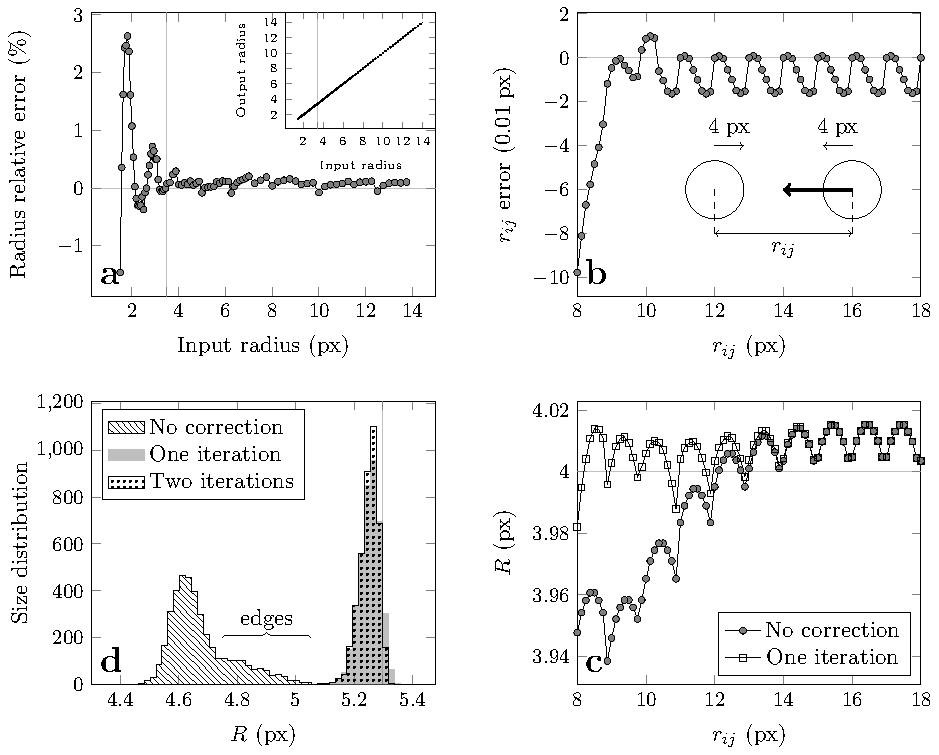
\includegraphics{generate-figure3.pdf}
\end{center}
	\caption{\textbf{Results from perfect images.} \textbf{a} Sizing of an isolated sphere. Left of the vertical line our algorithm uses a doubled image. \textbf{b} Localisation error and \textbf{c} sizing error function of the distance between two particles. Oscillations are due to off-lattice centre position. \textbf{d} Size distribution extracted from digitized configuration of 4000 monodisperse hard spheres at $0.50$ volume fraction (vertical line indicates the input radius). The tail to the right is due to particles on the edges of the image who have fewer neighbours and thus are more `dilute'. \textbf{c} and \textbf{d} also show the effect of finite dilution correction up to convergence.}
	\label{fig:perfect}
\end{figure*}

\begin{figure*}
\begin{center}
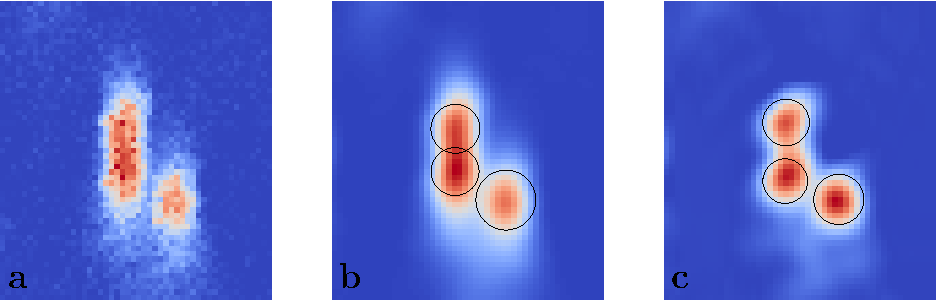
\includegraphics{generate-figure2.pdf}
\end{center}
	\caption{\textbf{Deconvolution.} Detail of the same $YZ$ slice of \textbf{a} original confocal image, \textbf{b} previous blurred by $\sigma_0=1.6$, \textbf{c} previous deconvolved by measured kernel (see text). Circles indicate the tracked particles position and size when using whether \textbf{b} or \textbf{c} as first Gaussian layer $G_0$. All three centres are in the slice $\pm \unit{0.5}{px}$}
	\label{fig:deconv}
\end{figure*}

\begin{figure*}
\begin{center}
\includegraphics{generate-figure1.pdf}
\end{center}
	\caption{\textbf{Sizing of our colloids.} \textbf{a,} Size distribution estimated \emph{in situ} (dashed line) by our multiscale algorithm ($\sim 1.7\times 10^6$ instantaneous sizing). Comparison with the size distribution estimated from \textsc{sem} of only $140$ dry particles (steps) is possible once $23\%$ of swelling of particle diameters is taken into account (full line). \textbf{b,} First peak of the radial distribution function with (full line) and without (dashed) the individual sizes data. Taking into account the measured sizes rectifies the effect of the polydispersity: the peak is thinner and higher.}
	\label{fig:sizing}
\end{figure*}

\end{document}